\chapter{Movement}\label{ch:move}
For our robot to be able to show the results of path finding,
it needed to be able to move.

We decided to move only along a simple 2D grid-like structure,
therefore wheels were the easiest solution.
\section{Motors}\label{sec:motors}
A stepper motor is a motor that moves one step at a time, with its step defined by a step angle.

\begin{figure}[h]
	\centering
	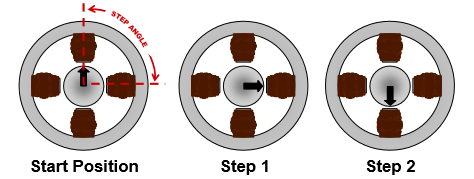
\includegraphics[width=\textwidth]{figures/motor1.png}
	\caption{Step Angle}
\end{figure}

The image above represents a stepper motor that requires 4 steps to complete a 360 degrees rotation. This determines the step angle to be 90 degrees. 
The main components of a stepper motor are represented in the image below, and they consist of stators, windings(phases), and rotor.
The part that moves, is the rotor, which can be magnetized or not, depending on the type of stepper motor.

\begin{figure}[h]
	\centering
	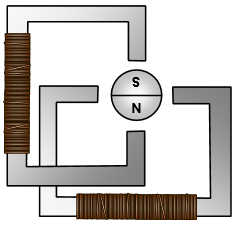
\includegraphics[width=0.5\textwidth]{figures/motor2.png}
	\caption{Main Components}
\end{figure}

By applying a voltage across one of the windings, current will start flowing through it. By using the right-hand rule, the direction of the magnetic flux can be determined. This is represented in the image below.

\begin{figure}[h]
	\centering
	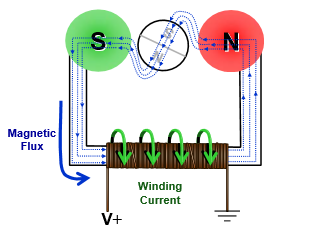
\includegraphics[width=0.6\textwidth]{figures/motor3.png}
	\caption{Direction of Magnetic Flux}
\end{figure}

The flux will want to travel through the path that has the least resistance. This determines the rotor to change its position to minimize resistance. This is shown in the image below.

\begin{figure}[h]
	\centering
	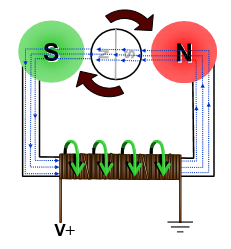
\includegraphics[width=0.5\textwidth]{figures/motor4.png}
	\caption{Direction of Magnetic Flux 2}
\end{figure}
\subsection{Types of Stepper Motors}
\subsubsection{Permanent Magnet Motor}
This type of stepper motor has a magnetized rotor. Each winding, will be subdivided into two, to better understand how to motor functions. The image below represents the windings, and how they are distributed inside a stepper motor.

\begin{figure}[htp] 
    \centering
    \subfloat[Rotor]{%
        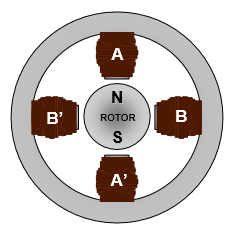
\includegraphics[width=0.4\textwidth]{figures/motor5.png}%
        }%
    \hfill%
    \subfloat[Winding]{%
        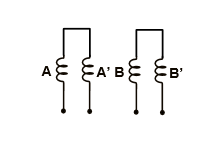
\includegraphics[width=0.4\textwidth]{figures/motor6.png}%
        }%
\end{figure}

\section{Motor Drivers}\label{sec:drivers}
\section{Wheels}\label{sec:wheels}
We wanted the robot to be capable of moving in eight directions from every position.
One solution for this would have been for the robot to turn every time it needed to change direction,
but since our goal was to test and time our path finding algorithm,
this was highly impractical.
One of our group members had worked with small wheel-based robots before,
and remembered omni-wheels.
\missingfigure{a picture of omniwheels}
Omni-wheels are wheels,
whose contact area consists of smaller wheels.
Those smaller wheels are able to spin freely,
with very little force needed.
If mounted in two pairs,
with the axes crossing at a 90 degree angle, \todo{find degree symbol}
one pair controls all forces along the x-axis,
and the other one along the y-axis.
\missingfigure{a figure of the forces in different directions added together}

\section{Direction Control}\label{sec:direction}
To control the direction of the robot,
we had to control which wheels turn how many degrees.

One option for this would have been to control each motor individually,
for this we would have needed four individually controllable stepper motors,
and four times four control outputs from our microcontroller.
This solution also meant precise timing between the four motors was needed,
in order to not generate any rotation.

We decided to look for a solution using less output pins,
and without the danger of rotation.

By analysing the requirements for our directional control,
we figured out that we only need 8 configurations of motor pairs.
\begin{center}
\begin{tabular}{|l|l|l|}
	\hline
	Direction & Pair A & Pair B	\\
	\hline
	North & forward & forward \\
	East 	& forward & backward \\
	South & backward & backward \\
	West 	& backward & forward \\
	\hline
	North-East & forward & off \\
	South-East & off & backward \\
	South-West & backward & off\\
	North-West & off & forward \\
	\hline
\end{tabular}
\begin{tabular}{|l|c|c|c|c|}
	\hline
	Direction & flipA & onA & flipB & onB \\
	\hline
	North & 0 & 1 & 0 & 1 \\
	East 	& 0 & 1 & 1 & 1 \\
	South & 1 & 1 & 1 & 1 \\
	West 	& 1 & 1 & 0 & 1 \\
	\hline
	North-East & 0 & 1 & 1 & 0 \\
	South-East & 1 & 0 & 0 & 1 \\
	South-West & 1 & 1 & 1 & 0 \\
	North-West & 1 & 0 & 1 & 1 \\
	\hline
\end{tabular}
\end{center}
\missingfigure{schematic of motor control circuit\label{fig:mot_ctrl}}

We decided to use 6 tri-state buffers as shown in figure\ref{fig:mot_ctrl}.
